% micromag user guide. Build from docs/: latexmk -pdf -outdir=<tmp> guide.tex, then copy guide.pdf here. Needs pgfplots (TeX Live has it).
% Keep it in step with docs/cards.md and docs/results.md: a changed card key or output changes this file too.
\documentclass[10pt,a4paper]{article}
\usepackage[T1]{fontenc}
\usepackage{newpxtext,newpxmath}
\usepackage[scaled=0.85]{beramono}
\usepackage[margin=2.2cm,top=2.4cm,bottom=2.4cm]{geometry}
\usepackage{microtype,booktabs,tabularx,graphicx,enumitem,xcolor,listings,caption,fancyhdr,titlesec}
\usepackage{pgfplots}
\pgfplotsset{compat=1.18}
\usepackage[hidelinks]{hyperref}

\definecolor{accent}{HTML}{1F4E79}
\definecolor{codebg}{HTML}{F4F6F8}
\definecolor{comment}{HTML}{5A6B7B}
\hypersetup{colorlinks=true,linkcolor=accent,urlcolor=accent,citecolor=accent}

\titleformat{\section}{\Large\bfseries\color{accent}}{\thesection}{0.6em}{}
\titleformat{\subsection}{\large\bfseries}{\thesubsection}{0.5em}{}
\titleformat{\subsubsection}{\normalsize\bfseries}{\thesubsubsection}{0.5em}{}
\titlespacing*{\section}{0pt}{14pt}{6pt}
\titlespacing*{\subsection}{0pt}{10pt}{4pt}

\setlist{itemsep=1pt,topsep=3pt,parsep=0pt}
\setlength{\parindent}{0pt}
\setlength{\parskip}{4pt}

\lstdefinelanguage{toml}{morecomment=[l]{\#},morestring=[b]",sensitive=true}
\lstset{basicstyle=\ttfamily\small,backgroundcolor=\color{codebg},frame=none,xleftmargin=4pt,xrightmargin=4pt,
  framexleftmargin=4pt,aboveskip=6pt,belowskip=6pt,columns=fullflexible,keepspaces=true,
  commentstyle=\color{comment},stringstyle=\color{accent!80!black},showstringspaces=false,breaklines=true}

\pagestyle{fancy}
\fancyhf{}
\fancyhead[L]{\small\color{comment}micromag user guide}
\fancyhead[R]{\small\color{comment}\nouppercase{\leftmark}}
\fancyfoot[C]{\small\thepage}
\renewcommand{\headrulewidth}{0.3pt}

\newcommand{\code}[1]{\texttt{#1}}
\newcommand{\mo}{\mu_0}
\newcommand{\vm}{\mathbf{m}}
\newcommand{\vH}{\mathbf{H}}
\newcommand{\kh}{\hat{\mathbf{k}}}
\newcommand{\dec}[1]{\textcolor{comment}{\small(#1)}}
\newcolumntype{Y}{>{\raggedright\arraybackslash}X}

\begin{document}

\begin{center}
  {\Huge\bfseries\color{accent} micromag}\\[4pt]
  {\Large A user's guide to the finite-difference micromagnetic solver}\\[6pt]
  {\small\color{comment} version 0.0.1 \quad$\cdot$\quad \href{https://github.com/tanooj-s/micromag}{github.com/tanooj-s/micromag} \quad$\cdot$\quad GPL-3.0-or-later}
\end{center}

\vspace{4pt}
\begin{figure}[h]
  \centering
  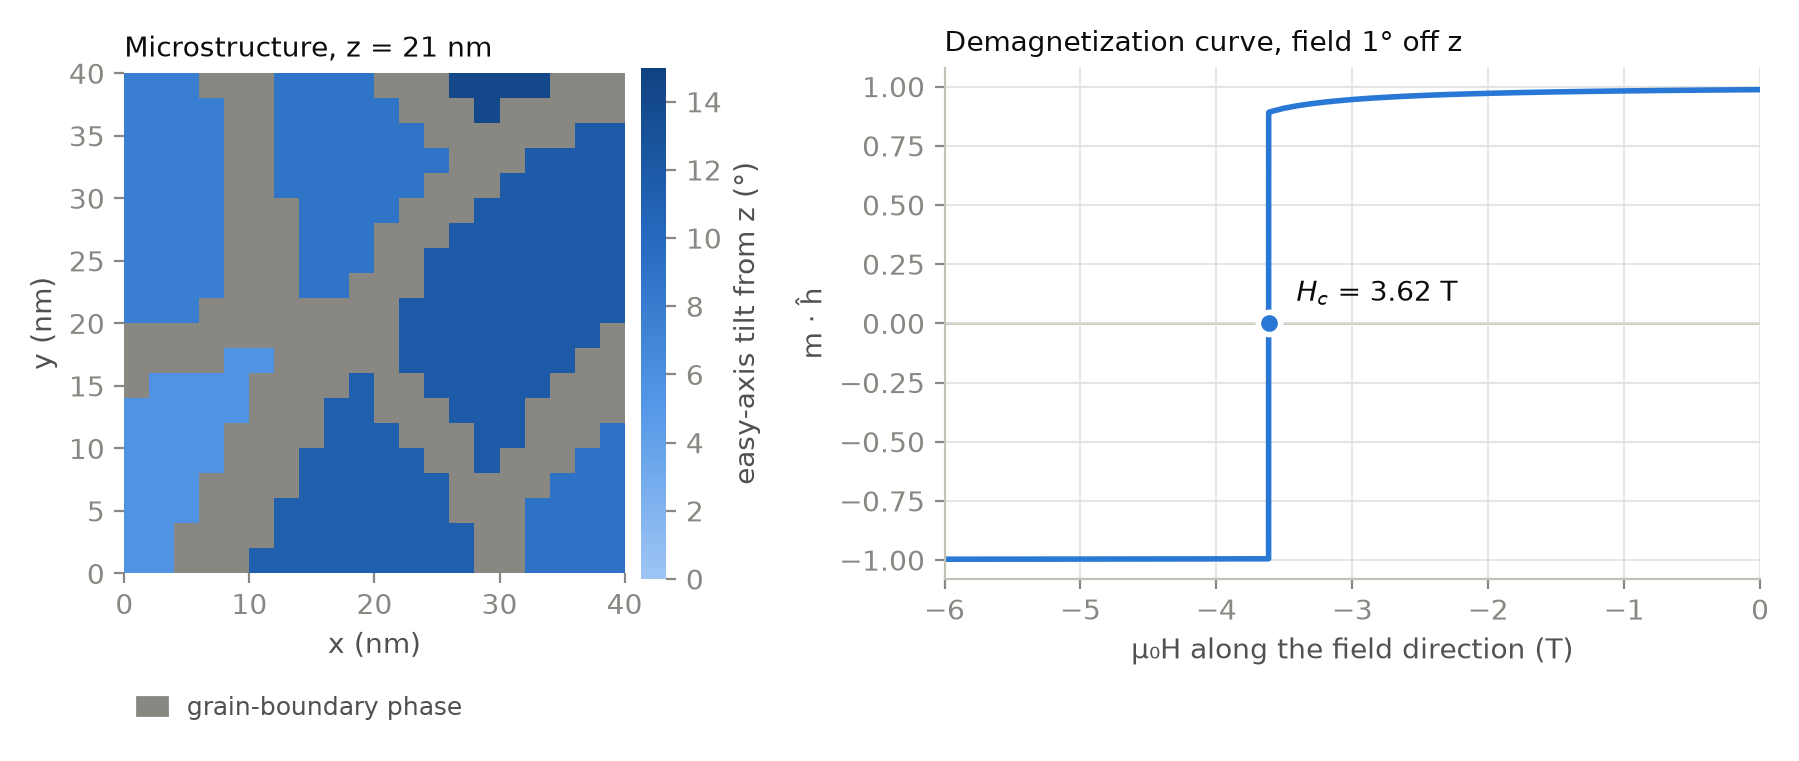
\includegraphics[width=\textwidth]{img/hero-light.png}
  \caption*{\small An 8-grain Nd$_2$Fe$_{14}$B polycrystal with a soft grain-boundary phase (left) and its demagnetisation
  curve (right), run from \code{examples/grains.toml} in about a minute on a laptop CPU.}
\end{figure}

\tableofcontents

% ---------------------------------------------------------------------------------------------------------------------
\section{What micromag is}

micromag computes how the magnetisation inside a small magnet, from a few nanometres to a few hundred, arranges itself
and moves. It divides the magnet into a regular grid of box-shaped cells, gives each cell a magnetisation direction
$\vm$ (a unit vector), and then either lets $\vm$ evolve in time or searches for the arrangement of lowest energy.

It is written from scratch in C++, with an optional CUDA backend, and driven from Python. It follows the micromagnetic
model of the review by Fischbacher \emph{et al.}\ (2018) \cite{fischbacher2018}, and its scope is modelled on the
micromagnetic part of MagTense. A simulation is described by one TOML file, the \emph{input card}, and produces one
results folder.

\textbf{What it can do.}
\begin{itemize}
  \item Four energy terms: exchange, uniaxial anisotropy, an applied (Zeeman) field and the magnetostatic (demagnetising)
        field, the last computed exactly from the Newell tensor by FFT.
  \item Four kinds of calculation: time evolution by the Landau--Lifshitz--Gilbert (LLG) equation, energy minimisation,
        quasi-static hysteresis sweeps with automatic refinement near switching, and energy barriers by geodesic NEB.
  \item A thermal field (Brown's stochastic field) for finite-temperature dynamics.
  \item Materials that vary cell by cell: named materials painted onto the grid as shapes, Voronoi polycrystals with
        per-grain easy axes and an optional grain-boundary phase, and exchange coupling set per pair of regions.
  \item Free or periodic boundaries on any axis, so a small tile can stand in for an extended film, a wire or bulk
        material.
  \item The same card on a CPU or an NVIDIA GPU, in double precision, with the same results on both (but see the GPU
        limit in Section~\ref{sec:validation}).
\end{itemize}

\textbf{What it does not do (yet).} Cubic or higher-order anisotropy, the Dzyaloshinskii--Moriya interaction,
magnetoelastic coupling, spatially varying applied fields or temperatures, and multi-GPU runs are not
implemented. For production research, the mature codes are mumax3, OOMMF, MagTense and Ubermag; micromag is a young code
validated against the standard benchmarks (Section~\ref{sec:validation}).

\textbf{Conventions.} SI units throughout: A/m, J/m, J/m$^3$, m, s, K. Applied fields in the card are given as
$\mo\vH$ in \emph{tesla}, because the literature quotes T and mT. Damping is the \emph{dimensionless Gilbert} $\alpha$.
Each design choice has a numbered entry D1, D2, \ldots{} in \code{DECISIONS.md}, with the alternatives that were
rejected; this guide cites them in grey, e.g.\ \dec{D11}.

% ---------------------------------------------------------------------------------------------------------------------
\section{Installing and running}

micromag builds from source with \href{https://docs.astral.sh/uv/}{uv}. You need a C++17 compiler; uv fetches Python
($\geq$ 3.11), CMake and the Python dependencies.
\begin{lstlisting}[language=bash]
git clone https://github.com/tanooj-s/micromag.git
cd micromag
uv sync                                     # CPU build
uv run micromag run examples/grains.toml -o runs/grains
\end{lstlisting}
The run prints one progress line per stage and writes \code{runs/grains/}. The output folder must be new or empty, so a
result is never overwritten.

\textbf{GPU build.} Install the CUDA toolkit (12.x or 13.x) with \code{nvcc} on \code{PATH}, then
\begin{lstlisting}[language=bash]
export SKBUILD_CMAKE_DEFINE="MICROMAG_CUDA=ON"
uv sync
uv run python -c "import micromag; print(micromag.has_cuda)"     # True
uv run micromag run examples/sp2.toml -o runs/sp2 --device cuda
\end{lstlisting}
Keep \code{SKBUILD\_CMAKE\_DEFINE} set in every later shell: \code{uv run} rebuilds when it changes, so forgetting it
silently rebuilds a CPU-only extension. Any NVIDIA GPU of compute capability 7.0 or newer works with CUDA 12 (7.5 with
CUDA 13). Because everything is float64, data-centre cards (V100, A100, H100) are much faster than consumer cards or the
T4. \code{docs/gpu.md} covers Google Colab and Slurm clusters.

\textbf{Apple Silicon.} If the \code{cmake} on \code{PATH} is an x86\_64 binary, \code{export ARCHFLAGS="-arch arm64"}
first, or the extension builds for the wrong architecture.

\textbf{Tests.} \code{uv run pytest} runs the fast suite (about a minute). \code{uv run pytest -m slow -s} runs the
physics benchmarks (about 15 minutes on a laptop CPU) and prints the comparisons.

% ---------------------------------------------------------------------------------------------------------------------
\section{The physical model}
\label{sec:model}

The state is the unit vector field $\vm(\mathbf{r}) = \mathbf{M}/M_s$. Each cell carries its own saturation
magnetisation $M_s$, exchange stiffness $A$, anisotropy constant $K$ and easy axis $\kh$. The total energy is the sum of
four terms, and each has an effective field $\vH = -\frac{1}{\mo M_s}\,\delta E/\delta\vm$ (Table~\ref{tab:terms}).

\begin{table}[h]
\centering\small
\caption{The energy terms. Equation numbers refer to Fischbacher \emph{et al.}\ (2018).}
\label{tab:terms}
\renewcommand{\arraystretch}{1.9}
\begin{tabularx}{\textwidth}{@{}l c >{$}l<{$} >{$}l<{$} Y@{}}
\toprule
Term & Eq. & \text{Energy density} & \text{Field } \vH & Parameters \\
\midrule
Exchange   & 8  & A\,|\nabla\vm|^2              & \dfrac{2}{\mo M_s}\nabla\cdot(A\nabla\vm)      & $A$ (J/m) \\
Anisotropy & 9  & -K(\vm\cdot\kh)^2             & \dfrac{2K}{\mo M_s}(\vm\cdot\kh)\,\kh           & $K$ (J/m$^3$), $\kh$ \\
Zeeman     & 11 & -\mo M_s\,\vm\cdot\vH_\mathrm{ext} & \vH_\mathrm{ext}                           & $\mo\vH_\mathrm{ext}$ (T), per stage \\
Demag      & 17--21 & -\tfrac12\mo M_s\,\vm\cdot\vH_d & \vH_d = -\mathcal{N} * (M_s\vm)            & none (geometry) \\
\bottomrule
\end{tabularx}
\end{table}

The anisotropy uses the paper's sign: a uniform $\vm \parallel \kh$ has energy $-KV$ \dec{D12}. $K > 0$ gives an easy
axis, $K < 0$ an easy plane. Vacuum is simply $M_s = 0$: such cells have no field, no energy and no exchange neighbours
\dec{D11}.

\textbf{Dynamics.} The LLG equation (eq.~25) is integrated in its Landau--Lifshitz form,
\[
  \frac{d\vm}{dt} = -\gamma'\,\vm\times\vH_\mathrm{eff} - \alpha\gamma'\,\vm\times(\vm\times\vH_\mathrm{eff}),
  \qquad \gamma' = \frac{\mo|\gamma|}{1+\alpha^2},
\]
with $\vH_\mathrm{eff}$ the sum of the four fields (plus the thermal field at $T>0$). The first term makes $\vm$ precess
about the field; the second, the damping, turns it towards the field. $\gamma$ defaults to $1.76086\times10^{11}$
rad/(T\,s).

\textbf{Equilibrium.} For slowly varying fields, as in a permanent magnet's hysteresis loop, the magnetisation sits in a
local energy minimum at each field (paper \S2.2.3). Equilibrium means zero torque, $\vm\times\vH_\mathrm{eff} = 0$, and
every stopping test in micromag is on the largest per-cell torque $\max|\vm\times\vH_\mathrm{eff}|/M_s$.

\textbf{Temperature.} Brown's model adds a Gaussian white-noise field $\vH_\mathrm{th}$ to $\vH_\mathrm{eff}$,
independent in every cell, component and step, with variance fixed by the fluctuation--dissipation theorem
\dec{D41}:
\[
  \sigma^2 = \frac{2\,\alpha\,k_B T}{\mo\,\gamma_0\,M_s\,V\,\Delta t}, \qquad \gamma_0 = \mo|\gamma|,
\]
where $V$ is the cell volume and $\Delta t$ the step. Larger damping needs stronger noise; a larger moment $M_sV$ needs
less. There is no $1+\alpha^2$ factor: the noise enters $\vH$ in Gilbert's form, as in mumax3.

% ---------------------------------------------------------------------------------------------------------------------
\section{The physics in more depth}
\label{sec:physics}

Section~\ref{sec:model} stated the model. This section explains where it comes from and what it predicts, using results
that can be worked out by hand. Most of them are also what the test suite compares the code against, so they double as
sanity checks for your own runs. The numbers use the two benchmark materials of Table~\ref{tab:scales}.

\subsection{From atoms to a continuum}
In a ferromagnet, the quantum-mechanical exchange interaction lines up neighbouring atomic moments. It is strong and
short-ranged, so the direction of the moments can only turn slowly from one atom to the next. Over a few lattice spacings
the moments can therefore be replaced by a smooth field $\mathbf{M}(\mathbf{r})$, which is the step that defines
micromagnetics (paper \S2.1). Well below the Curie temperature the \emph{length} of $\mathbf{M}$ stays at $M_s$ and only
its direction varies, which is why the state is a unit vector field and why every integrator renormalises $\vm$.

The model must resolve the transition inside a domain wall while staying coarser than the atoms. In a hard magnet that
wall is only about 4\,nm wide, so the continuum picture is working near its limit there.

The stable states of a magnet at a given field are the local minima of the energy $E[\vm]$ of eqs.~8--11. There are usually
many, and which one the magnet sits in depends on its history. That dependence is what gives a magnet its memory.

\subsection{What each energy term wants}
\textbf{Exchange} wants $\vm$ uniform and charges for gradients. A spiral $\vm = (\cos qx, \sin qx, 0)$ costs $Aq^2$ per
unit volume, so a twist twice as tight costs four times as much.

\textbf{Anisotropy} comes from the crystal, which through spin--orbit coupling favours some directions for $\vm$. The
uniaxial form $-K(\vm\cdot\kh)^2$ cannot tell $+\kh$ from $-\kh$. This gives two equally good minima, the ``up'' and
``down'' of a permanent magnet, and turning away from either by an angle $\theta$ costs $K\sin^2\theta$ per unit volume.

\textbf{Zeeman} energy is the applied field pulling $\vm$ towards itself. It is the only term that separates up from
down, and the only one linear in $\vm$.

\textbf{Demagnetising} energy is the magnet acting on itself. With no currents, $\nabla\times\vH_d = 0$ and
$\nabla\cdot\mathbf{B} = 0$ give $\nabla\cdot\vH_d = -\nabla\cdot\mathbf{M}$ (paper eqs.~12--15): the field behaves as
if it came from magnetic charges, of density $-\nabla\cdot\mathbf{M}$ in the volume and $\mathbf{M}\cdot\mathbf{n}$ on
the surface. Field lines run from the positive to the negative charges, so inside a uniformly magnetised body they
oppose $\mathbf{M}$, hence the name. The factor $\frac12$ in eq.~10 is there because this is a self-energy: each pair of
cells must be counted once. The energy equals $\frac{\mo}{2}\int\vH_d^2\,dV$ over all space, so it is never negative,
and it falls as charges are avoided. This is the one term that sees the whole magnet at once, and it drives $\vm$ to
lie along surfaces, to form closure patterns and to split into domains.

For a uniformly magnetised ellipsoid the field is uniform, $\vH_d = -N\mathbf{M}$, with demagnetising factors along the
three axes that sum to 1: $\frac13$ each for a sphere, $(0,0,1)$ for a thin film and $(\frac12,\frac12,0)$ for a long rod.
The periodic tests reproduce these limits \dec{D47}. Their energy $\frac12\mo N M_s^2$ per unit volume acts as a
\emph{shape anisotropy}. A film magnetised out of plane pays $\frac12\mo M_s^2$, so its effective anisotropy is
$K_\mathrm{eff} = K - \frac12\mo M_s^2$, and it only stays perpendicular if that is positive. Any body that is not an
ellipsoid, a cube included, has a non-uniform field that is strongest at its edges and corners, which matters below.

\subsection{Length scales}
Setting two energy densities equal gives the lengths that control a simulation. Exchange balances magnetostatics, $A/l^2
= \frac12\mo M_s^2$, at the exchange length $l_\mathrm{ex}$. Exchange balances anisotropy at the wall parameter
$\delta_0$. Their ratio squared is the quality factor (paper \S1.3):
\[
  l_\mathrm{ex} = \sqrt{\frac{2A}{\mo M_s^2}}, \qquad \delta_0 = \sqrt{\frac{A}{K}}, \qquad
  Q = \frac{2K}{\mo M_s^2} = \left(\frac{l_\mathrm{ex}}{\delta_0}\right)^2.
\]
With $Q\ll 1$ a material is soft: demag decides the pattern, and walls and vortices are set by $l_\mathrm{ex}$. With
$Q>1$ it is hard: anisotropy can hold $\vm$ against the worst possible demagnetising field, so a magnet of any shape is
possible, and $\delta_0$ is the shortest length. The paper's hardness parameter is $\kappa = K/(\mo M_s^2) = Q/2$, and
useful hard phases have $\kappa > 1$.

\textbf{One formula for every interaction.} Each term in the energy acts on $\vm$ like a field, and exchange resists that
field over a characteristic distance. A turn of $\vm$ over a length $l$ costs an exchange energy density of about $A/l^2$,
and a field $H$ offers about $\frac12\mo M_s H$. Setting them equal gives
\[
  l(H) = \sqrt{\frac{2A}{\mo M_s H}}.
\]
Put in the field of each interaction and the lengths above come out. Demag's largest field is $H = M_s$, which gives
$l_\mathrm{ex}$. Anisotropy's field is $H_K = 2K/(\mo M_s)$, which gives $\delta_0$. The applied field gives a third
length, which matters when the field is strong, as it is in a switching or barrier run. Temperature is the odd one out:
it is not a field, so compare energies instead. A block of side $l$ is held together by an exchange energy of about $Al$, which
equals $k_BT$ at $l_T = k_BT/A$. The shortest of the field lengths limits the mesh. $l_T$ sets no such limit: it marks the size at
which thermal energy rivals the exchange holding a block together, which is one way to see why thermal averages keep changing as
cells shrink (Section~\ref{sec:thermal}).

\textbf{Worked example: Nd$_2$Fe$_{14}$B.} These numbers are arithmetic on three measured inputs, which are not computed by
micromag. The review \cite{fischbacher2018} gives $\mo M_s = 1.61$\,T, $K = 4.3$\,MJ/m$^3$ and $A = 7.7$\,pJ/m at room
temperature. Then:
\begin{itemize}[nosep]
  \item $M_s = 1.61\,\mathrm{T}/\mo = 1.281$\,MA/m.
  \item The demag energy scale is $K_d = \frac12\mo M_s^2 = \frac12(1.61\,\mathrm{T})(1.281\,\mathrm{MA/m}) = 1.031$\,MJ/m$^3$.
  \item $l_\mathrm{ex} = \sqrt{A/K_d} = \sqrt{7.7\times10^{-12}/1.031\times10^{6}}\,\mathrm{m} = 2.73$\,nm.
  \item $\delta_0 = \sqrt{A/K} = \sqrt{7.7\times10^{-12}/4.3\times10^{6}}\,\mathrm{m} = 1.34$\,nm, so a wall is $\pi\delta_0 = 4.20$\,nm wide.
  \item $Q = K/K_d = 4.17$, and $\mo H_K = 2K/M_s = 6.71$\,T.
  \item At the $\mo H = 3.94$\,T of the barrier study, $l(H) = \sqrt{2A/(M_s\cdot 3.94\,\mathrm{T})} = 1.75$\,nm.
  \item At 300\,K, $l_T = k_BT/A = 0.54$\,nm.
\end{itemize}
Since $Q > 1$, $\delta_0$ is shorter than $l_\mathrm{ex}$, so anisotropy sets the scale here, not demag.

\begin{table}[h]
\centering\small
\caption{Derived quantities for the two benchmark materials: permalloy as in $\mu$MAG SP2 and SP4, and
Nd$_2$Fe$_{14}$B as in the 40\,nm cube.}
\label{tab:scales}
\begin{tabular}{@{}l l r r@{}}
\toprule
Quantity & Formula & Permalloy & Nd$_2$Fe$_{14}$B \\
\midrule
Polarisation & $\mo M_s$ & 1.005 T & 1.61 T \\
Exchange stiffness & $A$ & 13 pJ/m & 7.7 pJ/m \\
Anisotropy constant & $K$ & 0 & 4.3 MJ/m$^3$ \\
Exchange length & $l_\mathrm{ex}$ & 5.69 nm & 2.73 nm \\
Wall parameter & $\delta_0$ & none & 1.34 nm \\
Wall width & $\pi\delta_0$ & none & 4.20 nm \\
Wall energy & $\sigma = 4\sqrt{AK}$ & none & 23.0 mJ/m$^2$ \\
Quality factor & $Q$ & 0 & 4.17 \\
Anisotropy field & $\mo H_K = 2K/M_s$ & none & 6.71 T \\
\bottomrule
\end{tabular}
\end{table}

Table~\ref{tab:magnets} repeats the arithmetic for three other permanent-magnet phases. Only Nd$_2$Fe$_{14}$B has been simulated
in micromag; the other columns are reference values for planning a run.

\begin{table}[h]
\centering\small
\caption{Length scales of four permanent-magnet phases near room temperature. The first three rows are inputs from the
literature and the rest are computed from them. Nd$_2$Fe$_{14}$B: \cite{fischbacher2018}. SmCo$_5$: $M_s$ and $K$ from
\cite{coey2011}, $A$ from \cite{kurichenko}. Sm$_2$Co$_{17}$: \cite{yang2023}. SrFe$_{12}$O$_{19}$: $M_s$ and $K$ from
\cite{coey2011}, $A$ from \cite{murakami}.}
\label{tab:magnets}
\begin{tabular}{@{}l l r r r r@{}}
\toprule
Quantity & Formula & Nd$_2$Fe$_{14}$B & SmCo$_5$ & Sm$_2$Co$_{17}$ & SrFe$_{12}$O$_{19}$ \\
\midrule
Polarisation & $\mo M_s$ & 1.61 T & 1.08 T & 1.24 T & 0.48 T \\
Exchange stiffness & $A$ & 7.7 pJ/m & 12 pJ/m & 19.6 pJ/m & 10.7 pJ/m \\
Anisotropy constant & $K$ & 4.3 MJ/m$^3$ & 17.2 MJ/m$^3$ & 3.9 MJ/m$^3$ & 0.33 MJ/m$^3$ \\
\midrule
Demag energy scale & $K_d = \frac12\mo M_s^2$ & 1.03 MJ/m$^3$ & 0.46 MJ/m$^3$ & 0.61 MJ/m$^3$ & 0.09 MJ/m$^3$ \\
Anisotropy field & $\mo H_K$ & 6.7 T & 40 T & 7.9 T & 1.7 T \\
Quality factor & $Q = K/K_d$ & 4.2 & 37 & 6.4 & 3.6 \\
Exchange length & $l_\mathrm{ex}$ & 2.73 nm & 5.08 nm & 5.65 nm & 10.9 nm \\
Wall parameter & $\delta_0$ & 1.34 nm & 0.84 nm & 2.24 nm & 5.69 nm \\
Wall width & $\pi\delta_0$ & 4.20 nm & 2.62 nm & 7.04 nm & 17.9 nm \\
Wall energy & $\sigma = 4\sqrt{AK}$ & 23.0 mJ/m$^2$ & 57.5 mJ/m$^2$ & 35.0 mJ/m$^2$ & 7.5 mJ/m$^2$ \\
Thermal length, 300 K & $l_T = k_BT/A$ & 0.54 nm & 0.35 nm & 0.21 nm & 0.39 nm \\
\bottomrule
\end{tabular}
\end{table}

\textbf{How far to trust these inputs.} $M_s$ and $K$ are well measured, but $A$ is hard to measure and the published values
disagree, and each length goes as $\sqrt{A}$. For SmCo$_5$ the literature gives $A$ from 8.6 pJ/m \cite{yang2023} to 23.6 pJ/m
\cite{pierobon}, which moves $\delta_0$ from 0.71 to 1.17\,nm. For Sm$_2$Co$_{17}$, $A = 24.7$\,pJ/m and $K = 3.3$\,MJ/m$^3$
\cite{pierobon} give $\delta_0 = 2.74$\,nm. For the ferrite, an older $A = 6$\,pJ/m \cite{sfofilm} gives $\delta_0 = 4.26$\,nm.
The ferrite's newer value has a direct check: its $\pi\delta_0 = 17.9$\,nm matches the measured wall width of
$17.8\pm1.4$\,nm \cite{murakami}. Also, $K = 4.9$\,MJ/m$^3$ is often quoted for Nd$_2$Fe$_{14}$B, and the review uses both
values. Commercial Sm$_2$Co$_{17}$ is a cell structure with a SmCo$_5$-like boundary phase, so one column does not describe a
real 2:17 magnet. SmCo$_5$'s $\delta_0$ is only about two unit cells, so a continuum model is near its limit there.

\subsection{Domain walls}
Take a wall across which $\vm$ turns by $\theta(x)$ from one easy direction to the other, staying in the plane of the
wall so that $\nabla\cdot\mathbf{M} = 0$ and no charges appear (a Bloch wall). The energy per unit area is $\int
(A\theta'^2 + K\sin^2\theta)\,dx$. Exchange wants the turn spread out, anisotropy wants it short, and the minimum has
the two densities equal at every point, $A\theta'^2 = K\sin^2\theta$. Integrating this gives
\[
  \theta(x) = 2\arctan e^{x/\delta_0}, \qquad m_z = \cos\theta = -\tanh(x/\delta_0), \qquad
  \sigma = \int 2K\sin^2\theta\,dx = 4\sqrt{AK}.
\]
The profile is in Figure~\ref{fig:physics}(a). The width $\pi\delta_0$ is the distance the turn would take at its
steepest slope. The tests place this exact profile on the grid and require the torque to vanish and the energy to reach
$\sigma$ at second order in $\Delta x$ \dec{D13}. It is also why a hard-magnet mesh needs cells of about 1\,nm: a coarser
wall is pinned between cells, and the coercive field comes out too high.

Walls cost energy, so a magnet only forms them when the demag energy saved is larger. The saving grows with volume and
the cost with area, so below some size a particle stays in one domain. The textbook estimate for a sphere is a radius of
$36\sqrt{AK}/(\mo M_s^2)$, about 100\,nm for Nd$_2$Fe$_{14}$B. Keeping grains near or below this size is one reason
fine-grained magnets have higher coercivity.

\begin{figure}[t]
\centering
\pgfplotsset{phys/.style={width=0.315\textwidth,height=4.4cm,axis lines=left,tick align=outside,
  tick style={color=comment},axis line style={color=comment},every tick label/.style={font=\scriptsize},
  label style={font=\footnotesize},title style={font=\footnotesize,yshift=-3pt},
  every axis plot/.append style={line width=1pt}}}
\begin{tikzpicture}[baseline]
\begin{axis}[phys,title={(a) Bloch wall},xlabel={$x/\delta_0$},ylabel={component of $\vm$},xmin=-5,xmax=5,ymin=-1.1,ymax=1.1,
  ytick={-1,0,1},xtick={-4,-2,0,2,4}]
  \addplot[accent,domain=-5:5,samples=81,mark=none] {-tanh(x)};
  \addplot[comment,dashed,domain=-5:5,samples=81,mark=none] {1/cosh(x)};
  \node[font=\scriptsize,anchor=south] at (axis cs:-3.2,0.55) {$m_z$};
  \node[font=\scriptsize,anchor=west] at (axis cs:1.6,0.62) {$m_y$};
\end{axis}
\end{tikzpicture}%
\hfill
\begin{tikzpicture}[baseline]
\begin{axis}[phys,title={(b) Macrospin, field against $\vm$},xlabel={angle $\varphi$ from the start ($^\circ$)},
  ylabel={$(E-E_0)/KV$},xmin=0,xmax=180,ymin=-1.5,ymax=1.45,xtick={0,90,180},ytick={-1,0,1}]
  \addplot[accent!30,domain=0:180,samples=91,mark=none] {sin(x)^2};
  \addplot[accent!55,domain=0:180,samples=91,mark=none] {sin(x)^2+0.6*cos(x)-0.6};
  \addplot[accent!80,domain=0:180,samples=91,mark=none] {sin(x)^2+1.2*cos(x)-1.2};
  \addplot[accent,domain=0:180,samples=91,mark=none] {sin(x)^2+2*cos(x)-2};
  \node[font=\scriptsize,anchor=south] at (axis cs:90,1.0) {$h=0$};
  \node[font=\scriptsize,anchor=west] at (axis cs:100,0.28) {0.3};
  \node[font=\scriptsize] at (axis cs:64,-0.16) {0.6};
  \node[font=\scriptsize,anchor=east] at (axis cs:78,-0.95) {1};
\end{axis}
\end{tikzpicture}%
\hfill
\begin{tikzpicture}[baseline]
\begin{axis}[phys,title={(c) 40\,nm cube, 300 K},xlabel={$\mo|H|$ (T)},ylabel={$E_B/k_BT$},xmin=3.5,xmax=5.5,ymin=0,ymax=32,
  xtick={3.5,4,4.5,5,5.5},ytick={0,10,25}]
  \addplot[comment,dashed,line width=0.6pt,mark=none] coordinates {(3.5,25) (5.5,25)};
  \addplot[comment,dotted,line width=0.8pt,mark=none] coordinates {(5.275,0) (5.275,32)};
  \addplot[accent,mark=*,mark size=1.6pt,mark options={solid,fill=accent}] coordinates
    {(3.7,28.604) (3.94,22.478) (4.2,16.877) (5.2,0.703)};
  \node[font=\scriptsize,anchor=south] at (axis cs:4.55,25) {25 $k_BT$};
  \node[font=\scriptsize,anchor=east] at (axis cs:5.26,13) {static};
\end{axis}
\end{tikzpicture}
\caption{(a) The exact wall profile. (b) A macrospin's energy against its angle, with the field along the axis and
opposing $\vm$, at $h = H/H_K$ of 0, 0.3, 0.6 and 1. The barrier is $(1-h)^2KV$ and is gone at $h=1$. (c) Barriers computed
by \code{gneb} for the cube, $30^3$ cells, field $1^\circ$ off the axis, against the static switching field of 5.275\,T.}
\label{fig:physics}
\end{figure}

\subsection{Coherent rotation: the Stoner--Wohlfarth model}
In a particle small enough that exchange keeps $\vm$ uniform, one angle $\varphi$ describes the state. With the field at
an angle $\psi$ to the easy axis, the energy per unit volume is (paper \S2.2.5)
\[
  \frac{E}{V} = K\sin^2\varphi - \mo M_s H\cos(\varphi-\psi).
\]
At low field there are two minima separated by a maximum (Figure~\ref{fig:physics}b). As an opposing field grows, the
minimum $\vm$ sits in becomes shallower, until it merges with the maximum and $\vm$ has to jump. Asking where the first
and second derivatives vanish together gives the switching field, the Stoner--Wohlfarth astroid \cite{stoner}:
\[
  \frac{H_\mathrm{sw}(\psi)}{H_K} = \left(\cos^{2/3}\psi + \sin^{2/3}\psi\right)^{-3/2}, \qquad H_K = \frac{2K}{\mo M_s}.
\]
It is 1 on the axis, and only $\frac12$ at $45^\circ$, because a tilted field also exerts a torque on $\vm$. It already
drops to 0.907 at $1^\circ$, which is why a small misalignment matters so much. With the field on the axis the barrier
is exactly $E_B = KV(1-h)^2$ with $h = H/H_K$; off the axis it falls as $(1-H/H_\mathrm{sw})^{3/2}$ near switching \cite{victora}. The
minimiser tests use the astroid and the \code{gneb} tests use the barrier.

\textbf{From one grain to a loop.} A hysteresis loop is the sequence of local minima the magnet passes through as the
field changes (paper \S2.2.1). The remanence $M_r$ is $\langle\vm\rangle$ along the field at $H=0$, and the coercive
field $H_c$ is the field where it crosses zero. An ensemble of non-interacting Stoner--Wohlfarth grains with random axes
has $M_r = 0.5\,M_s$ and $H_c = 0.479\,H_K$, a further check \dec{D37}.

\subsection{Why real magnets switch early}
The cube of Table~\ref{tab:scales} has $\mo H_K = 6.71$\,T, or 6.09\,T at $1^\circ$ off the axis, but it switches at
5.275\,T, and the 25\,nm core--shell cube at 2.72\,T. Real magnets do worse still. That the ideal coercive field is
never reached is called Brown's paradox (paper \S1.3). The reason is that reversal does not need every cell to turn
together. A small reversed \emph{nucleus} forms where it is easiest, at a corner with a strong local demagnetising
field or in a soft defect, and once its wall can move, it sweeps through the grain. The paper's summary is its eq.~7:
\[
  H_c = \alpha_K\,\alpha_\psi\,H_N - N_\mathrm{eff}M_s - H_f.
\]
$H_N$ is the ideal nucleation field. $\alpha_\psi$ covers misaligned grains and $\alpha_K$ soft defects, which can reduce
$H_c$ as far as $H_N/4$. $N_\mathrm{eff}$ covers local demagnetising fields, and $H_f$ thermal activation. The paper's
60\,nm polycrystal gives $\mo H_N = 6.7$\,T, $\alpha_\psi = 0.71$, $\alpha_K = 0.67$, $N_\mathrm{eff} = 0.2$ and
$\mo H_f = 0.23$\,T.

A simulation can switch these effects on one at a time, which no experiment can. In micromag, grain axes in \code{[grains]}
set the misalignment, a \code{boundary} phase or a soft \code{[[region]]} adds defects, \code{demag = false} removes the
magnetostatics, and a \code{gneb} stage gives the thermal part.

\subsection{Dynamics: precession and damping}
A magnetic moment carries angular momentum, so a field does not pull it straight round: it exerts a torque, and $\vm$
precesses like a tilted spinning top, $d\vm/dt = -\gamma_0\,\vm\times\vH_\mathrm{eff}$ with $\gamma_0 = \mo|\gamma|$. The
frequency is $|\gamma|/2\pi = 28.0$\,GHz per tesla of $\mo H$, or about 190\,GHz (a period near 5\,ps) in the 6.7\,T
anisotropy field of Nd$_2$Fe$_{14}$B. This motion is always perpendicular to the field, so on its own it conserves
energy, and a test holds the code to that at $\alpha=0$ \dec{D20}.

Gilbert \cite{gilbert} added a friction term proportional to the velocity:
\[
  \frac{d\vm}{dt} = -\gamma_0\,\vm\times\vH_\mathrm{eff} + \alpha\,\vm\times\frac{d\vm}{dt}.
\]
Taking $\vm\times$ of this and substituting it back gives the Landau--Lifshitz form of Section~\ref{sec:model}, and that
is where the $1+\alpha^2$ comes from. For one cell, the energy then falls at the rate
\[
  \frac{dE}{dt} = -\mo M_s V\,\alpha\gamma'\,|\vm\times\vH_\mathrm{eff}|^2 \leq 0,
\]
so it stops falling exactly when the torque vanishes. Physical damping is small ($\alpha = 0.02$ in SP4), so $\vm$
spirals in over many turns. With so little friction it can swing past a nearby minimum and end in a different one, which
is why \code{llg-dynamics} and \code{minimize} may disagree from the same start. For coherent rotation the fastest
reversal is at $\alpha = 1$. In the limit of large damping only the second term survives, and that term is the direction
of steepest descent (paper \S2.2.4), which is the link between the LLG equation and the minimiser.

\subsection{Temperature, barriers and rare events}
At temperature $T$, a magnet in equilibrium visits a state with probability proportional to $e^{-E/k_BT}$. Damping
alone would drain all the energy, so the thermal field must feed it back at exactly the rate that keeps this
distribution, and that requirement fixes $\sigma^2$ in Section~\ref{sec:model}: the fluctuation--dissipation theorem. The
tests check it directly, with an ensemble of macrospins against the Boltzmann distribution, and against the Langevin
curve $\coth x - 1/x$ with $x = \mo M_s V H/k_BT$ at $K=0$ \dec{D44}.

Crossing a barrier $E_B$ is a rare event, with a waiting time given by the Arrhenius--N\'eel law
\[
  \tau = \frac{1}{f_0}\,e^{E_B/k_BT},
\]
where the attempt frequency $f_0$ is typically $10^9$ to $10^{11}$\,Hz. A wait of one second then needs $E_B\approx
25\,k_BT$ (exactly so for $f_0 \approx 7\times10^{10}$\,Hz), the paper's criterion for coercivity at room temperature. The
exponential makes this sharp: 5 $k_BT$ more or less changes the wait by a factor of about 150, and 40 $k_BT$ means about
a month. A particle whose whole barrier $KV$ is below 25 $k_BT$ flips by itself and shows no remanence, which is
superparamagnetism. For Nd$_2$Fe$_{14}$B at 300\,K that is a cube of edge below about 3\,nm.

\textbf{Why barriers need their own method.} The relevant barrier is the lowest pass between two states. A
\emph{minimum energy path} is one along which the energy gradient is parallel to the path, and its highest point is a
saddle: a maximum along the path and a minimum across it. A direct thermal run would have to wait for the event, at
about $10^{15}$ femtosecond steps per second of magnet time, while \code{gneb} goes straight to the saddle.

\textbf{Nucleation sets the barrier, not the volume.} The 40\,nm cube has $KV \approx 66{,}000\,k_BT$, and coherent
rotation at 3.94\,T would still need about $11{,}000\,k_BT$ \dec{D48}. The computed barrier there is 22.5 $k_BT$
(Figure~\ref{fig:physics}c), because the saddle is a small reversed nucleus. As a rough estimate, 25 $k_BT$ buys
only about 4.5\,nm$^2$ of wall at $\sigma = 23$\,mJ/m$^2$, a patch about 2\,nm across. A wire with free ends shows the
same physics in closed form: a wall entering at the end has a barrier that tends to $4\sqrt{AK}\,S$ at low field, with $S$
the wire's cross-section, however long the wire is. The \code{gneb} tests compare against that formula \dec{D51}.

Thermal activation lowers the cube's coercive field from 5.275\,T to 3.841\,T, a drop of 27\%. The paper quotes up to
25\% for nearly ideal particles like this, and only 8\% for its magnet with a soft grain boundary, where defects have
already taken the easy reversal route.

% ---------------------------------------------------------------------------------------------------------------------
\section{Implementation choices}

This section explains the numerical choices a user should know about, because they set accuracy, cost and the limits
of what can be simulated.

\subsection{Grid and data layout}
\label{sec:layout}
The grid is a box of $n_x\times n_y\times n_z$ cells of size $\Delta x\times\Delta y\times\Delta z$. Coordinates in the
card are measured in metres from the lower corner; cell $(i,j,k)$ is centred at
$((i+\frac12)\Delta x, (j+\frac12)\Delta y, (k+\frac12)\Delta z)$. All arrays are float64 \emph{structure-of-arrays}:
vectors are shaped \code{(3, nz, ny, nx)} and scalars \code{(nz, ny, nx)}, with $x$ fastest \dec{D9}. This layout feeds
the FFTs and the GPU directly. Every material parameter is stored per cell, so the solver core never knows about shapes
or grains: geometry is expanded into per-cell arrays in Python, and new geometry never touches C++.

\subsection{Exchange}
A second-order six-neighbour Laplacian \dec{D11}. The coupling across a face between two cells uses the
\emph{harmonic mean} $A_\mathrm{face} = 2A_1A_2/(A_1+A_2)$, which is zero if either side is zero, so a hard grain cannot
couple straight through a non-magnetic boundary. The surfaces are free (Neumann): a missing or vacuum neighbour
contributes nothing. Across faces between two different regions, $A_\mathrm{face}$ can be scaled or replaced by a
\code{[[coupling]]} entry \dec{D35}, which models thin, weak interfaces without resolving them with cells. On a periodic
axis the neighbour across the boundary is the cell on the opposite face \dec{D45}.

\subsection{Demagnetising field}
The demagnetising field is a convolution of the magnetisation with the demagnetisation tensor $\mathcal{N}$, which
depends only on the offset between two cells \dec{D14, D15}.
\begin{itemize}
  \item \textbf{Tensor.} The exact Newell formulas for cell pairs closer than 20 cells; beyond that, a point-dipole kernel
        averaged over $3\times3\times3$ Gauss points in each cell, because Newell's formulas lose precision far away
        (they sum 27 large, nearly cancelling terms). The tensor is accurate to about $10^{-6}$ relative, far below the
        $O(\Delta x^2)$ discretisation error. Cells flatter than about 1:4 are untested.
  \item \textbf{Convolution.} Zero-padded to $2n$ per free axis (an axis with $n=1$ stays at 1) and done with real-to-complex
        FFTs: pocketfft on the CPU, cuFFT on the GPU. The tensor's spectrum is computed once per run.
  \item \textbf{Cost.} The padding makes demag the dominant cost in memory and time: about $8\times$ the cell count per
        padded array. Cell counts with small prime factors transform fastest.
  \item \textbf{Switch.} \code{demag = false} in \code{[grid]} removes the term, e.g.\ for Stoner--Wohlfarth comparisons
        \dec{D36}.
\end{itemize}

\subsection{Periodic boundaries}
\code{pbc = [Px, Py, Pz]} makes an axis periodic, with $P$ copies of the tile on each side, as in mumax3's
\code{SetPBC} \dec{D45}. The exchange neighbour wraps around, and Voronoi grains continue across the boundary.
For demag, a periodic axis is not padded, so the FFT's own wrap-around is used on purpose, and each tensor entry sums
the copies in a window centred on each cell: every cell sees $(2P+1)$ tile lengths of material, with the two end
layers at half weight when $n$ is even. The copies are a \emph{finite} block on purpose: in 2D and 3D, the field of an
infinite lattice of copies depends on the shape of the body they fill, so the shape is made explicit. Each copy uses
the same Newell and dipole kernels. The sum costs about 1\,s for $128\times128\times1$ cells at $P=10$ and about 20\,s
for $64^3$ cells at $P=5$, once per run. The error left by a finite $P$ shrinks slowly: halving with each doubling of
$P$ for a film, and falling 4$\times$ for a rod.

\subsection{Time integration}
\begin{itemize}
  \item \textbf{\code{rk45}} (default at $T=0$). An adaptive Dormand--Prince 5(4) integrator \dec{D18}. The error is
        the largest per-cell $|\vm_5-\vm_4|$, so a few fast-switching cells in a large grid are not averaged away. A step
        is rejected when the error exceeds \code{tol}; the next step is $h\cdot0.9(\mathrm{tol}/\mathrm{err})^{1/5}$,
        clamped to 0.2--5$\times$. $\vm$ is renormalised after every accepted step. Six field evaluations per step.
  \item \textbf{\code{heun}} (default at $T>0$). A fixed step \code{dt}. One noise sample per step, held over the
        predictor and the corrector, which converges to Brown's (Stratonovich) equation \dec{D42}. Two field
        evaluations per step.
  \item \textbf{\code{rk23}}. Adaptive Bogacki--Shampine 3(2) with the noise frozen over each step. When a step is
        rejected, its random increment is \emph{not} thrown away (that would favour steps where the noise happened to be
        small and bias the temperature); an exact Brownian bridge splits it between the shorter retry and the rest.
        Three field evaluations per step.
\end{itemize}
The random numbers come from a counter-based Philox4x32-10 generator, written once and shared by the CPU and GPU, keyed
by the stage's \code{seed} and its position in the card. The same card and seed give the same run on either device.

\subsection{Energy minimisation and hysteresis}
\code{minimize} is projected steepest descent with Barzilai--Borwein step sizes (eqs.~22--23, Exl \emph{et al.}\ 2014;
essentially mumax3's minimiser) \dec{D21}. The direction is $-\vm\times(\vm\times\vH)$, the update is renormalised, and
the step alternates the two BB formulas with no line search. The energy may rise on single iterations; convergence is
judged by the torque only. If \code{max\_iter} is reached the stage fails, so a half-converged state near a switching
field is never reported silently.

A \code{hysteresis} stage minimises at each field of a sweep. With \code{refine\_to}, a coarse step that crosses
$\vm\cdot\hat{\mathbf{h}}=0$ or makes $\langle\vm\rangle$ jump is undone and halved, recursively, down to
\code{refine\_to} \dec{D31}. A loop then costs about 45 field steps instead of about 600, with the switch still resolved
finely.

\subsection{Energy barriers}
A \code{gneb} stage finds the minimum energy path between a state and its reverse, by geodesic NEB with a climbing image
(Bessarab \emph{et al.}\ 2015) \cite{bessarab} \dec{D48}. A chain of images feels the true force across the path and a spring along it;
the highest image climbs to the saddle, so the barrier needs no interpolation. Distances are Ms-weighted rms great-circle
angles. The first path is a great circle with $10^{-2}$ rad of noise per cell, since a perfectly uniform path can't
leave itself. L-BFGS moves the whole chain with no line search, as the forces are not the gradient of any energy
(Ivanov \emph{et al.}\ 2020) \cite{ivanov} \dec{D49}. Each step rotates the cells, and no cell may turn more than 0.1 rad: an rms cap
lets a small nucleus turn as far as it likes. While the path's energy range exceeds 10 barriers, its far end moves in to
the first image lower than the start, because a pass of 25 $k_BT$ on a slope of $10^5$ $k_BT$ would fit between two
images.

\subsection{Backends}
The drivers (step control, BB steps, refinement) are written once. The per-cell arithmetic sits behind a small backend
interface with two implementations: the CPU backend, which is the reference ``oracle'', and the CUDA backend, one thread
per entry, with cuFFT and CUB \dec{D24}. Every CUDA kernel is tested against the CPU. Within a call, $\vm$ stays on the
device; it is copied to and from the host only at the start and end of a \code{run\_until} or \code{minimize}. There is
no global state, so several problems can coexist in one Python process.

% ---------------------------------------------------------------------------------------------------------------------
\section{Kinds of simulations}

A card has a few setup sections, then an ordered list of stages. The magnetisation carries over from one stage to the
next; the applied field does \emph{not}: every stage states its own field, defaulting to zero. Table~\ref{tab:sims} maps
common questions to stage types.

\begin{table}[h]
\centering\small
\caption{Typical simulations and how to set them up.}
\label{tab:sims}
\begin{tabularx}{\textwidth}{@{}>{\raggedright\arraybackslash}p{3.6cm} >{\raggedright\arraybackslash}p{3.3cm} Y@{}}
\toprule
Question & Stage(s) & Notes and example \\
\midrule
What is the ground state or a metastable state? & \code{minimize} & Fastest route to equilibrium. Start from several initial
  states and compare energies (as in $\mu$MAG SP3, flower vs vortex). \\
How does $\vm$ move in time? & \code{llg-dynamics} with \code{duration} & Physical $\alpha$ and $\gamma$; sample with
  \code{sample\_every}. Example: \code{examples/sp4.toml} (switching a permalloy film). \\
Relax with real dynamics & \code{llg-dynamics} with \code{until\_torque} & Large $\alpha$ (e.g.\ 1); stops when the
  torque is small. Used for SP4's S-state. \\
Coercivity, remanence, switching field & \code{hysteresis} & Quasi-static sweep with \code{refine\_to}; summary
  \code{Hc\_T}, \code{switch\_T}, \code{remanence}. Examples: \code{sp2.toml}, \code{cube\_core\_shell.toml}. \\
Microstructure effects & \code{hysteresis} + \code{[grains]}, \code{[[region]]}, \code{[[coupling]]} & Grains, boundary
  phases, soft shells, weak interfaces. Example: \code{grains.toml}. \\
Thermal fluctuations, superparamagnetism & \code{llg-dynamics} with \code{temperature} & \code{heun} or \code{rk23};
  noisy time series of $\langle\vm\rangle$. Barriers of a few $k_BT$ only (Section~\ref{sec:thermal}). \\
Energy barriers, thermal coercivity & \code{gneb} & The barrier against field, and where it crosses 25 $k_BT$. Reaches
  barriers no thermal run can. Check with a second \code{seed}. \\
Bulk or extended material & \code{[grid] pbc = [P, P, P]} & A periodic tile without an artificial outer surface;
  check the result at two values of $P$. \\
Continue from an earlier result & \code{[initial] file = ...} & Restart from any saved state, even on a different cell
  size. \\
\bottomrule
\end{tabularx}
\end{table}

\textbf{A full hysteresis loop} is two \code{hysteresis} stages, one sweeping down and one back up.
\textbf{A field slightly off the easy axis} (e.g.\ 1$^\circ$) is the convention for hard-magnet cubes: exactly along the
axis, the reversed state is an exact but unstable equilibrium that a minimiser may never leave.

\textbf{Example: $\mu$MAG standard problem 4}, relax then switch (\code{examples/sp4.toml}):
\begin{lstlisting}[language=toml]
[grid]
n    = [128, 32, 1]                    # cells along x, y, z
cell = [3.90625e-9, 3.90625e-9, 3e-9]  # m

[material.permalloy]
Ms = 8e5        # A/m
A  = 1.3e-11    # J/m

[initial]
m = [1, 1, 1]   # normalised on load

[[stage]]       # the S-state: damped dynamics until the torque is small
type = "llg-dynamics"
alpha = 1.0
gamma = 1.759457895880903e11   # rad/(T s), as muMAG specifies
tol = 1e-9                     # well below until_torque
until_torque = 1e-6
check_every = 50e-12
max_duration = 20e-9

[[stage]]       # the reversal, sampled every 1 ps
type = "llg-dynamics"
alpha = 0.02
gamma = 1.759457895880903e11
mu0_H = [-24.6e-3, 4.3e-3, 0.0]   # T
duration = 1e-9
sample_every = 1e-12
\end{lstlisting}

\textbf{Example: a polycrystal} (\code{examples/grains.toml}, abridged): eight Nd$_2$Fe$_{14}$B grains with axes within
15$^\circ$ of $z$, coated by a 4\,nm soft phase, swept to $-6$\,T.
\begin{lstlisting}[language=toml]
[grid]
n    = [20, 20, 20]
cell = [2e-9, 2e-9, 2e-9]

[material.grain]            # listed first: region 0, the background
Ms = 1281197.29             # A/m (mu0 Ms = 1.61 T)
A  = 8e-12
K  = 4.9e6

[material.boundary]
Ms = 379584.54              # A/m (mu0 Ms = 0.477 T)
A  = 6.12e-12

[grains]
count    = 8
first_id = 1
material = "grain"
seed     = 1
axes     = { mean = [0, 0, 1], cone_deg = 15 }
boundary = { thickness = 4e-9, material = "boundary", id = 100 }

[initial]
m = [0.0174524, 0.0, 0.9998477]

[[stage]]
type       = "hysteresis"
direction  = [0.0174524, 0.0, 0.9998477]   # 1 degree off z
mu0_H_from = 0.0
mu0_H_to   = -6.0
mu0_H_step = 0.1
refine_to  = 1e-3
\end{lstlisting}

% ---------------------------------------------------------------------------------------------------------------------
\section{Input card reference}
\label{sec:cards}

Validation is strict and happens before anything runs: an unknown key, a missing key or a wrong type is an error, and
every problem in the card is reported together. ``req.''\ marks a required key.

\subsection{Top level and \code{[grid]}}
\begin{tabularx}{\textwidth}{@{}l l l Y@{}}
\toprule
Key & Type & Default & Meaning \\
\midrule
\code{device} & string & \code{"cpu"} & \code{"cpu"} or \code{"cuda"}; \code{--device} on the command line overrides it \\
\code{n} & 3 integers $\geq 1$ & req. & cells along $x, y, z$ \\
\code{cell} & 3 numbers $>0$ & req. & cell size (m) \\
\code{demag} & bool & \code{true} & include the demagnetising field \\
\code{pbc} & 3 integers $\geq0$ & \code{[0,0,0]} & periodic copies per side along $x, y, z$; 0 is a free axis \\
\bottomrule
\end{tabularx}

\subsection{\code{[material.<name>]}}
One or more named materials. The \emph{first} one listed fills the whole grid as region~0, the background. The name
\code{vacuum} is built in ($M_s=0$) and reserved.

\begin{tabularx}{\textwidth}{@{}l l l Y@{}}
\toprule
Key & Type & Default & Meaning \\
\midrule
\code{Ms} & number $\geq 0$ & req. & saturation magnetisation (A/m); 0 is vacuum \\
\code{A} & number $\geq 0$ & req. & exchange stiffness (J/m) \\
\code{K} & number & 0 & uniaxial anisotropy (J/m$^3$); energy $-K(\vm\cdot\kh)^2$ \\
\code{axis} & 3 numbers & \code{[0,0,1]} & easy axis $\kh$, normalised on load \\
\bottomrule
\end{tabularx}

\subsection{\code{[[region]]}: painted shapes}
Regions are painted in card order, and later paints win. A cell belongs to a shape if its \emph{centre} is inside it.
The region map is \code{uint8}, so ids run from 0 to 255.

\begin{tabularx}{\textwidth}{@{}l l l Y@{}}
\toprule
Key & Type & Default & Meaning \\
\midrule
\code{id} & integer 1--255 & req. & region id (0 is the background) \\
\code{material} & string & req. & a defined material or \code{"vacuum"} \\
\code{shape} & string & req. & \code{all}, \code{cuboid}, \code{cylinder} or \code{ellipsoid} \\
\code{inverse} & bool & \code{false} & paint everything \emph{outside} the shape \\
\code{axis} & 3 numbers & material's & override the easy axis in this region \\
\midrule
\multicolumn{4}{@{}l}{\emph{Shape keys}} \\
\code{cuboid} & \multicolumn{3}{Y}{\code{corners = [[x0,y0,z0],[x1,y1,z1]]}; lower bounds inside, upper outside} \\
\code{cylinder} & \multicolumn{3}{Y}{\code{center}, \code{radius}, \code{height}; axis along $z$} \\
\code{ellipsoid} & \multicolumn{3}{Y}{\code{center}, \code{semi\_axes = [a,b,c]}} \\
\bottomrule
\end{tabularx}

The results record each region's exact volume next to its painted volume, and warn when they differ by more than 5\%,
which catches shapes clipped by the grid or too coarsely resolved. To make a sphere, paint \code{vacuum} with an
\code{ellipsoid} and \code{inverse = true}.

\subsection{\code{[grains]}: Voronoi polycrystals}
Optional, applied after all \code{[[region]]} painting. It fills one region with 3D Voronoi grains: each cell joins the
grain of its nearest seed. Seeds are drawn uniformly over the box, so the grains do not depend on the cell size.

\begin{tabularx}{\textwidth}{@{}l l l Y@{}}
\toprule
Key & Type & Default & Meaning \\
\midrule
\code{count} & integer $\geq1$ & req. & number of grains \\
\code{first\_id} & integer 1--255 & req. & grains get ids \code{first\_id} \ldots{} \code{first\_id+count-1} ($\leq 255$) \\
\code{material} & string & req. & the grains' material \\
\code{seed} & integer $\geq0$ & req. & same seed, same grains and axes \\
\code{within} & region id & 0 & the region to fill \\
\code{axes} & see text & \code{"material"} & easy axis per grain \\
\code{boundary} & table & none & grain-boundary phase \\
\bottomrule
\end{tabularx}

\code{axes} is \code{"material"} (every grain uses the material's axis), \code{"random"} (isotropic), or
\code{\{ mean = [x,y,z], cone\_deg = $\theta$ \}} (uniform within $\theta$ of the mean, $0<\theta\leq90$).
\code{boundary = \{ thickness = t, material = "...", id = n \}} coats each grain face: a cell closer than $t/2$ to its
grain's boundary joins region $n$, so neighbouring grains are separated by $t$. The distance is computed exactly from the
bisecting planes between seeds. $t$ must be at least two cells; thinner boundaries are modelled with \code{[[coupling]]}.
On a periodic axis the grains use minimum-image distances and continue across the boundary; painted shapes do not wrap.

\subsection{\code{[[coupling]]}: exchange between regions}
{\sloppy Rescales the exchange across faces between two regions, as mumax3's \code{ext\_ScaleExchange} and
\code{ext\_InterExchange} do. Exchange inside a region is unchanged; later entries win.\par}

\begin{tabularx}{\textwidth}{@{}l l Y@{}}
\toprule
Key & Type & Meaning \\
\midrule
\code{regions} & \code{[a, b]} & two region ids, or \code{"grains"} for every grain id; $a\neq b$.
  \code{["grains","grains"]} means every pair of distinct grains \\
\code{scale} & number $\geq0$ & multiplies the harmonic-mean $A$ across those faces \\
\code{A} & number $\geq0$ & sets the face exchange (J/m) directly \\
\bottomrule
\end{tabularx}
Give exactly one of \code{scale} or \code{A}. \code{scale = 0} decouples the regions completely.

\subsection{\code{[initial]}}
Exactly one of \code{m = [x, y, z]} (a uniform start, normalised) or \code{file = "path/trajectory.h5"} (relative to
the card) with an optional \code{state}: \code{"final"} (default) or \code{"stage<k>"}, the last snapshot of stage $k$.
A restart needs the same cell counts \code{n}; the cell size may differ. The file's SHA-256 goes into the provenance.

\subsection{\code{[[stage]]}, \code{type = "minimize"}}
\begin{tabularx}{\textwidth}{@{}l l Y@{}}
\toprule
Key & Default & Meaning \\
\midrule
\code{mu0\_H} & \code{[0,0,0]} & applied field (T) \\
\code{torque\_tol} & \code{1e-6} & stop when $\max|\vm\times\vH|/M_s$ falls below this \\
\code{max\_iter} & \code{100000} & fail after this many iterations \\
\bottomrule
\end{tabularx}

\subsection{\code{[[stage]]}, \code{type = "hysteresis"}}
\begin{tabularx}{\textwidth}{@{}l l Y@{}}
\toprule
Key & Default & Meaning \\
\midrule
\code{direction} & req. & field direction, normalised \\
\code{mu0\_H\_from}, \code{mu0\_H\_to} & req. & field range along \code{direction} (T), inclusive \\
\code{mu0\_H\_step} & req. & step (T); must divide the range into whole steps \\
\code{torque\_tol}, \code{max\_iter} & \code{1e-6}, \code{100000} & as for \code{minimize} \\
\code{refine\_to} & none & halve any step that crosses $\vm\cdot\hat{\mathbf h}=0$ or jumps, down to this (T) \\
\code{refine\_jump} & \code{0.1} & a change $|\Delta\langle\vm\rangle|$ above this counts as a jump \\
\code{dump} & \code{false} & save a snapshot at every field, not just the last \\
\bottomrule
\end{tabularx}

The stage reports \code{Hc\_T}, the first zero of $\vm\cdot\hat{\mathbf h}$ (linearly interpolated); \code{switch\_T},
the midpoint of the largest jump; and \code{remanence}, $\langle\vm\rangle$ at zero field if the sweep passes through it.

\subsection{\code{[[stage]]}, \code{type = "gneb"}}
\begin{tabularx}{\textwidth}{@{}l l Y@{}}
\toprule
Key & Default & Meaning \\
\midrule
\code{direction} & req. & field direction, normalised \\
\code{mu0\_H} & req. & list of field values along \code{direction} (T), one path each, in order \\
\code{images} & 20 & images on the path, counting both ends; at least 3 \\
\code{temperature} & 300 & temperature (K), which sets $k_BT$ in the summary \\
\code{torque\_tol} & \code{1e-4} & stop when $\max|\text{force}|/M_s$ is below this on every image \\
\code{max\_iter} & \code{100000} & give up after this many iterations (the stage fails) \\
\code{seed} & 0 & seeds the small noise on the first path \\
\bottomrule
\end{tabularx}

At each field the stage minimises the current $\vm$ and $-\vm$ as the two end states, then finds the path. It leaves
$\vm$ at the last field's start state. It reports \code{barrier\_J} and \code{barrier\_kT} per field, and \code{Hc\_T},
where the barrier crosses 25 $k_BT$ (linearly interpolated), or \code{null}. A run can converge to a higher saddle than
the lowest, so re-run with another \code{seed} and keep the lowest. A saved path may end just past the saddle.

\subsection{\code{[[stage]]}, \code{type = "llg-dynamics"}}
\begin{tabularx}{\textwidth}{@{}l l Y@{}}
\toprule
Key & Default & Meaning \\
\midrule
\code{alpha} & req. & Gilbert damping (dimensionless) \\
\code{gamma} & \code{1.76086e11} & gyromagnetic ratio (rad/(T\,s)) \\
\code{mu0\_H} & \code{[0,0,0]} & applied field (T) \\
\code{method} & \code{rk45} ($T=0$), \code{heun} ($T>0$) & \code{rk45} ($T=0$ only), \code{heun} (fixed step) or \code{rk23} (adaptive) \\
\code{tol} & \code{1e-6} & per-step error tolerance (\code{rk45}, \code{rk23}) \\
\code{max\_step} & none & largest step (s) (\code{rk45}, \code{rk23}) \\
\code{dt} & req.\ for \code{heun} & fixed step (s); only with \code{heun} \\
\code{temperature} & 0 & temperature (K) \\
\code{seed} & req.\ at $T>0$ & noise seed, an integer $0$ to $2^{32}-1$ \\
\code{dump\_every} & none & snapshot interval (s) \\
\midrule
\multicolumn{3}{@{}l}{\emph{Stopping rule: exactly one of}} \\
\code{duration} & & run time (s), with optional \code{sample\_every} (s) for table rows \\
\code{until\_torque} & & stop when $\max|\vm\times\vH|/M_s$ is below this; needs \code{check\_every} and
  \code{max\_duration} (s), and \code{tol} $\leq$ \code{until\_torque}/100. Refused at $T>0$ \\
\bottomrule
\end{tabularx}

% ---------------------------------------------------------------------------------------------------------------------
\section{Choosing numerical parameters}

micromag never picks the cell size, the step or the tolerances for you. These rules of thumb come from the benchmarks.

\textbf{Cell size.} A cell must be smaller than the shortest length over which $\vm$ turns. Two lengths matter:
the exchange length $l_\mathrm{ex} = \sqrt{2A/(\mo M_s^2)}$, which sets vortex and flux-closure structures, and the
wall parameter $\delta_0 = \sqrt{A/K}$ (a Bloch wall is $\pi\delta_0$ wide), which matters in hard magnets. For
permalloy, $l_\mathrm{ex}\approx 5.7$\,nm; for Nd$_2$Fe$_{14}$B, $l_\mathrm{ex}\approx 2.7$\,nm and
$\delta_0\approx 1.3$\,nm. The benchmarks used $0.5\,l_\mathrm{ex}$ for $\mu$MAG SP2, $0.7\,l_\mathrm{ex}$ for SP4, and
1--1.3\,nm for the Nd$_2$Fe$_{14}$B cubes. In the hard-magnet benchmarks, coarser meshes gave higher coercive fields, so
\textbf{check any result by refining the mesh once}. Keep cells close to cubic; aspect ratios beyond 1:4 are untested
for the demag tensor.

\textbf{How fine depends on what you measure.} No single cell size suits every result (lengths from
Section~\ref{sec:physics}, Table~\ref{tab:magnets}):
\begin{itemize}[nosep]
  \item \emph{Coercive field.} The review's finite-element cubes, spheres and polycrystals changed by less than 2\% between
        1.3 and 2.7\,nm at the surface \cite{fischbacher2018}, so about $2\delta_0$ can be enough for Nd$_2$Fe$_{14}$B. It asks
        for cells below $l_\mathrm{ex}$ where the nucleus forms: the transverse demag field diverges at corners and edges.
  \item \emph{Wall energy and a wall-type barrier.} The wire's barrier error is second order: $-0.35\%$ at $0.28\,\delta_0$ and $-1.4\%$
        at $0.57\,\delta_0$, about $-4.4\%\times(\Delta x/\delta_0)^2$ \dec{D51}. That gives about $-4\%$ at $\delta_0$, an extrapolation
        beyond the measured range.
  \item \emph{A barrier set by a small nucleus.} The most demanding case measured so far. The 40\,nm cube at 3.94\,T extrapolates to about
        24.1\,$k_BT$ and reads about $-7\%\times(\Delta x/\delta_0)^2$ from $0.75\,\delta_0$ to $1.2\,\delta_0$. At $2\delta_0$ that law
        breaks down: the barrier is 41\% low and the path turns into a staircase (Section~\ref{sec:coarse}).
  \item \emph{Thermal averages.} These do not converge as the mesh is refined (Section~\ref{sec:thermal}).
\end{itemize}
For a barrier there is a second test besides $\delta_0$: \textbf{the nucleus at the saddle must span several cells}. The cube's
nucleus is about 17\,nm$^3$ at 3.94\,T on every mesh from $25^3$ to $40^3$. Four reversed cells at $25^3$ were enough for a clean
single pass; at $15^3$ one cell (19\,nm$^3$) is bigger than the nucleus, and the path broke up. A stronger field should shrink the
nucleus, as $l(H)$ suggests, so check this at the field you care about.

Table~\ref{tab:mesh} turns this into starting values for each magnet. They are starting values, not guarantees: only the
Nd$_2$Fe$_{14}$B column has been run, and on a single problem. A $\delta_0$ cell leaves only about three cells across a wall.

\begin{table}[h]
\centering\small
\caption{Starting cell sizes from Table~\ref{tab:magnets}. A cell of $\delta_0$ gives an error of about 4\% on the wire and 7\% on the
cube's barrier; a cell of $\delta_0/2$ gives about 1\% and 2\%. The last row is the cost of a 40\,nm cube at $\delta_0$.}
\label{tab:mesh}
\begin{tabular}{@{}l r r r r@{}}
\toprule
& Nd$_2$Fe$_{14}$B & SmCo$_5$ & Sm$_2$Co$_{17}$ & SrFe$_{12}$O$_{19}$ \\
\midrule
Shortest length & $\delta_0$ & $\delta_0$ & $\delta_0$ & $\delta_0$ \\
Coarsest cell for walls and barriers, $\delta_0$ & 1.34 nm & 0.84 nm & 2.24 nm & 5.69 nm \\
Cell for 1--2\%, $\delta_0/2$ & 0.67 nm & 0.42 nm & 1.12 nm & 2.85 nm \\
Coarsest cell for a nucleation field, $l_\mathrm{ex}$ & 2.73 nm & 5.08 nm & 5.65 nm & 10.9 nm \\
40\,nm cube at $\delta_0$ & $30^3$ & $48^3$ & $18^3$ & $7^3$ \\
\bottomrule
\end{tabular}
\end{table}

In a soft material ($Q\ll 1$) the same logic gives $l_\mathrm{ex}$ as the limit. With several materials on one grid, as in a
core--shell cube, take the shortest length of any phase that $\vm$ turns in.

\textbf{Grid size.} Memory and time are dominated by the demag FFT on a grid padded to $2n$ per free axis. On a laptop CPU,
$10^4$--$10^5$ cells are practical; $10^6$ cells (e.g.\ a 100\,nm cube at 1\,nm) belong on a GPU.

\textbf{LLG tolerances.} \code{tol} bounds the per-step change of $\vm$ in any cell; $10^{-6}$ is fine for trajectories.
To stop on torque, \code{tol} must sit at least 100$\times$ below \code{until\_torque}: each step's error re-excites a
torque of a few $\times$ \code{tol}, so the threshold would otherwise never be reached. For relaxation, a large
$\alpha$ ($\approx 1$) is fastest; it is unphysical for the path but not for the end state.

\textbf{Minimiser tolerance.} \code{torque\_tol = 1e-6} (in units of $M_s$) is the tested default. Near a switching
field, convergence slows, so leave \code{max\_iter} generous rather than loosening the tolerance.

\textbf{Hysteresis steps.} Use a coarse \code{mu0\_H\_step} (about 1--5\% of the expected switching field) with a fine
\code{refine\_to} (about $10^{-3}$\,T for hard magnets, $10^{-5}$\,T for soft films). The coarse step must divide the
range exactly.

\textbf{Energy barriers.} The 40\,nm cube used 10 images at the default \code{torque\_tol = 1e-4}; check a barrier by doubling
\code{images} and with a second \code{seed}. Run a long wire at a small field, not zero, where a wall has no single
saddle. Convergence can depend on the mesh: a $15^3$ cube of 2.67\,nm cells often failed within 2000 iterations where $8^3$, $12^3$ and
$30^3$ converged \dec{D49}. A chain that converges has not proved it found the highest pass (Section~\ref{sec:coarse}).

\textbf{Thermal step \code{dt} (for \code{heun}).} It must resolve the fastest precession: about 1/80 of
$2\pi(1+\alpha^2)/(\gamma_0 H_\mathrm{max})$, where $H_\mathrm{max}$ includes the exchange field, up to
$12\cdot 2A/(\mo M_s\Delta x^2)$ on a 3D grid. At 1/20, Heun's bias on a coupled film is about 2\% \dec{D52}. It should also be well below a cell's free-diffusion time
$\tau_N = (1+\alpha^2)\mo M_s V/(2\alpha\gamma_0 k_BT)$; the tests use $\tau_N/200$. Check a result by halving
\code{dt} once. Femtosecond steps are typical.

% ---------------------------------------------------------------------------------------------------------------------
\subsection{Case study: a barrier on a coarse mesh}
\label{sec:coarse}
The same 40\,nm Nd$_2$Fe$_{14}$B cube at $\mo H = -3.94$\,T, 1$^\circ$ off $z$, was run on meshes from $15^3$ (cells of 2.67\,nm, $2\delta_0$) to $40^3$ (1.00\,nm, $0.75\,\delta_0$). From $25^3$ up the chain converged on
every seed. At $15^3$ it usually did not. The studies are in \code{benchmarks/saddle\_finish.pdf} \dec{D54} and
\code{benchmarks/barrier\_cell\_size.pdf} \dec{D56}.

\textbf{The tool.} Because the field is linear in $\vm$, the exact curvature of the energy on the spheres costs one field
evaluation per direction: $A v = -P(L v) + (\vm\cdot\vH)v$, where $L$ is the field without $H_\mathrm{ext}$ and $P$ removes the
component along $\vm$. So Newton's method can be run on one state, with MINRES solving each step. It finds the nearest point of zero
force, of any kind. Counting the negative curvatures tells which kind: none is a minimum, one is a saddle, more is not a
pass. Pushing a saddle both ways along its negative mode and relaxing shows which minima it joins, though about one push in seven
overshot to the far side. This tool lives in \code{benchmarks/barrier\_cell\_size.py}, not in the \code{gneb} stage. It was tried as
a way to speed up \code{gneb} and dropped: L-BFGS gets the barrier right, and the saving was too small.

\begin{figure}[h]
\centering
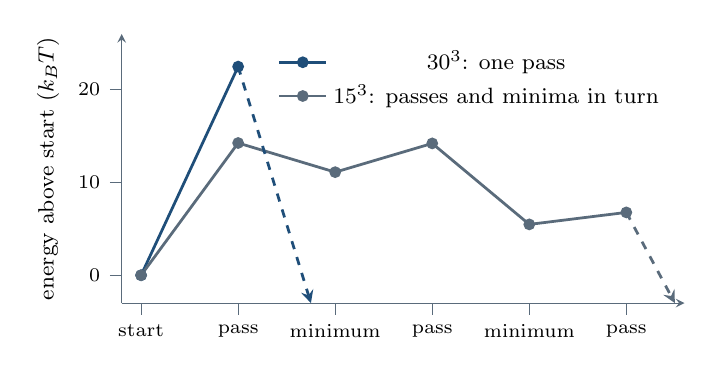
\begin{tikzpicture}
\begin{axis}[width=0.72\textwidth,height=5cm,axis lines=left,tick align=outside,tick style={color=comment},
  axis line style={color=comment},every tick label/.style={font=\scriptsize},label style={font=\footnotesize},
  ylabel={energy above start ($k_BT$)},xtick={0,1,2,3,4,5},xticklabels={start,pass,minimum,pass,minimum,pass},
  xmin=-0.2,xmax=5.6,ymin=-3,ymax=26,legend style={draw=none,font=\footnotesize,at={(0.98,0.98)},anchor=north east},
  every axis plot/.append style={line width=1pt}]
\addplot[accent,mark=*,mark size=1.6pt] coordinates {(0,0)(1,22.478)};
\addlegendentry{$30^3$: one pass}
\addplot[comment,mark=*,mark size=1.6pt] coordinates {(0,0)(1,14.249)(2,11.107)(3,14.203)(4,5.478)(5,6.770)};
\addlegendentry{$15^3$: passes and minima in turn}
\addplot[accent,dashed,-stealth] coordinates {(1,22.478)(1.75,-3)};
\addplot[comment,dashed,-stealth] coordinates {(5,6.770)(5.5,-3)};
\end{axis}
\end{tikzpicture}
\caption{Stationary points of the cube at 3.94\,T, each joined to the next by a push and relax. Dashed arrows lead on down to the
reversed state, about 156,000\,$k_BT$ below the start.}
\label{fig:stairs}
\end{figure}

\textbf{What it found.} At $30^3$ every finish reached 22.4783\,$k_BT$, the chain's own value to four decimals, with one
negative mode ($-1.64$\,T, the next $+0.86$\,T), in 18--53 field evaluations after a chain of 3,600--7,700. At $15^3$ the path is a
staircase (Figure~\ref{fig:stairs}). The first pass at 14.249\,$k_BT$ leads to a minimum at 11.107\,$k_BT$ with one reversed cell,
then a second pass at 14.203\,$k_BT$. The climbing image has two tops 0.05\,$k_BT$ apart to choose between, and chains that did
converge often stopped on the lower one. The likely cause is that a nucleus smaller than one cell cannot grow smoothly, so
reversal proceeds cell by cell.

\textbf{Refining the mesh.} From $25^3$ to $40^3$ all 12 chains converged, seeds agreed to four decimals, and Newton from all 96 images
found one pass or the start, so the staircase is gone by $1.2\,\delta_0$. The odd meshes $25^3$ and $35^3$ behave like the even ones, so
odd $n$ is not the cause. Iterations stayed at 540--1020 with no trend, so the mesh does not slow L-BFGS.
\begin{center}\small
\begin{tabular}{@{}l r r r r r r@{}}
\toprule
Mesh & Cell (nm) & Cell$/\delta_0$ & Converged & Barrier ($k_BT$) & Against 24.1 & Nucleus \\
\midrule
$15^3$ & 2.67 & 1.99 & 0 of 3 & 14.249 & $-41\%$ & under 1 cell \\
$25^3$ & 1.60 & 1.20 & 3 of 3 & 21.695 & $-10\%$ & 4 cells, 16.4\,nm$^3$ \\
$30^3$ & 1.33 & 1.00 & 3 of 3 & 22.478 & $-7\%$ & 7 cells, 16.6\,nm$^3$ \\
$35^3$ & 1.14 & 0.85 & 3 of 3 & 22.891 & $-5\%$ & 11 cells, 16.4\,nm$^3$ \\
$40^3$ & 1.00 & 0.75 & 3 of 3 & 23.158 & $-4\%$ & 17 cells, 17.0\,nm$^3$ \\
\bottomrule
\end{tabular}
\end{center}
The barrier rises as $E_0 - c\,\Delta x^2$, with $E_0 = 24.0$--24.1\,$k_BT$ depending on which meshes are fitted. That is an
extrapolation below the finest cell run. It would move our 25\,$k_BT$ crossing from 3.84\,T to about 3.91\,T, close to the published
3.94\,T (an estimate, using the slope measured at $30^3$). Meshes between $15^3$ and $25^3$ were not run, so the exact point where the
staircase starts is unknown, and why $8^3$ and $12^3$ converged is unexplained.

\textbf{The starting path is not the cause.} Three other first paths gave the same picture at $15^3$, with 3 seeds and 2000 iterations
each:
\begin{center}\small
\begin{tabular}{@{}l c c l@{}}
\toprule
First path & Converged at $10^{-4}$ & Converged at $10^{-2}$ & Barrier when converged ($k_BT$) \\
\midrule
Great circle (the default) & 0 of 3 & 1 of 3 & 14.2025 \\
The $30^3$ path, coarsened & 0 of 3 & 1 of 3 & 14.2492 \\
A corner nucleus, grown along the path & 0 of 3 & 0 of 3 & none \\
An LLG reversal at $-7$\,T & 0 of 3 & 2 of 3 & 14.2025, 14.2025 \\
\bottomrule
\end{tabular}
\end{center}
The great-circle start converges at $30^3$, and Newton found the same points from every start, so they belong to the discrete
landscape. A shift of 0.005\,$k_BT$ in the start state was enough to change which chains converged.

\textbf{What to take from it.} Non-convergence is the visible symptom, but the larger error is silent: a chain that converges at $15^3$
reports a barrier about 41\% low, and even a clean $30^3$ run reads 7\% low. Keep cells at or below $\delta_0$, make sure the nucleus spans
several cells, and compare at least two meshes before quoting a barrier.

\section{Thermal runs: what to expect}
\label{sec:thermal}

Set \code{temperature} (and \code{seed}) on an \code{llg-dynamics} stage:
\begin{lstlisting}[language=toml]
[[stage]]
type = "llg-dynamics"
alpha = 0.1
temperature = 300     # K
seed = 1              # same card and seed: the same run, on the CPU or the GPU
dt = 1e-14            # s, the fixed heun step; check by halving it
duration = 1e-9
sample_every = 1e-12
\end{lstlisting}
\begin{itemize}
  \item \textbf{Reach.} Steps resolve precession on femtosecond scales, so direct runs reach nanoseconds to microseconds.
        Thermally activated reversal over a 25\,$k_BT$ barrier (about a second) is far out of reach; use barriers of a
        few $k_BT$.
  \item \textbf{Cell-size dependence.} Each cell gets an independent kick, so smaller cells carry shorter-wavelength
        fluctuations and the magnet looks ``more thermal''. No correction is applied; report the cell size with any
        thermal result and compare at least two.
  \item \textbf{Double counting.} Parameters measured at temperature, such as $M_s(300\,\mathrm K)$, already contain
        the average effect of sub-cell fluctuations, and the noise adds them again. micromag does not correct for this.
  \item \textbf{Scope.} One temperature per stage, uniform in space. \code{minimize} and \code{hysteresis} are always
        at $T=0$. Each stage keys its noise by \code{seed} and its position in the card, so two stages with the same
        seed draw different numbers.
\end{itemize}

% ---------------------------------------------------------------------------------------------------------------------
\section{The results folder}

\code{micromag run CARD -o DIR} writes:\\
\begin{minipage}{\linewidth}
\begin{lstlisting}
DIR/
  card.toml                  the card, copied byte for byte
  provenance.json            versions, git state, timings, status, per-stage summaries
  git.diff                   only if the checkout had uncommitted changes
  stage1_llg-dynamics.csv    one table per stage: stage<k>_<type>.csv
  trajectory.h5              magnetisation snapshots and the region map
  trajectory.xdmf            sidecar for opening trajectory.h5 in ParaView
\end{lstlisting}
\end{minipage}

\textbf{Stage tables.} One row per sample, flushed as written (\code{tail -f} works). Time restarts at 0 in each stage.
\begin{itemize}
  \item \code{llg-dynamics}: \code{t, mu0\_Hx, mu0\_Hy, mu0\_Hz, mx, my, mz, E\_exchange, E\_anisotropy, E\_zeeman,
        E\_demag, E\_total, steps, rejected}
  \item \code{minimize}, \code{hysteresis}: the same without \code{t}, \code{steps} and \code{rejected}, plus
        \code{iterations}.
  \item \code{gneb}: \code{mu0\_Hx, mu0\_Hy, mu0\_Hz, image, s, E\_total, climbing}, one row per image per field.
\end{itemize}
$\langle\vm\rangle$ is averaged over magnetic cells only; energies are in J, fields in T, time in s. A refined
hysteresis stage revisits fields, and every field it computed is a row, in the order computed.

\textbf{\code{trajectory.h5}} (float64, gzip-compressed):
\code{/regions} is the \code{uint8} region map with a JSON \code{materials} attribute; \code{/stage<k>/m} holds the
snapshots, shaped \code{(count, 3, nz, ny, nx)}, with \code{/stage<k>/t} or \code{/stage<k>/mu0\_H}; \code{/final/m}
is the end state; \code{/failed/m} the last state of a failed stage. By default each stage saves its final snapshot;
\code{dump\_every} or \code{dump = true} saves more; a \code{gneb} stage saves every image of every field. Open \code{trajectory.xdmf} in ParaView (XDMF Reader) to view
$\vm$ and the regions over all snapshots.

\textbf{\code{provenance.json}} records the status (\code{running}, \code{completed} or \code{failed}, with the error),
timestamps, device and GPU name, package versions, the git hash and dirty flag, the initial state, each region's exact
and painted volume, and per stage its wall time, the hysteresis or \code{gneb} summary, or the LLG method, step counts, seed and
temperature. It is rewritten after each stage, so a killed run shows how far it got.

\textbf{Failures.} A stage fails at \code{max\_duration} or \code{max\_iter}, or on a solver error. The run stops, keeps
everything written so far, saves the last state in \code{/failed}, and exits with code 1. A bad card or a non-empty
output folder exits with code 2 before anything is written.

% ---------------------------------------------------------------------------------------------------------------------
\section{The Python API}

Everything a card does is available from Python, for scripting parameter studies or custom analysis. Arrays must be
float64 and C-contiguous in the layout of Section~\ref{sec:layout}; a wrong dtype or shape raises an error rather than silently
copying.
\begin{lstlisting}[language=Python]
import numpy as np
import micromag as mm

g = mm.Grid(64, 64, 1, 2e-9, 2e-9, 2e-9)         # nx, ny, nz, dx, dy, dz; pbc=(Px, Py, Pz)
s = (g.nz, g.ny, g.nx)
Ms, A, K = np.full(s, 8e5), np.full(s, 1.3e-11), np.zeros(s)
k = np.zeros((3, *s)); k[2] = 1
prob = mm.Problem(g, Ms, A, K, k, (0, 0, 0), device="cpu")   # H_ext in A/m; or "cuda"

m = np.zeros((3, *s)); m[0] = 1
mm.Minimizer(prob).minimize(m, torque_tol=1e-6)   # m is updated in place
print(prob.energies(m))                           # {"exchange": ..., "demag": ...} in J

llg = mm.LLG(prob, alpha=0.02)                    # gamma, tol, max_step, method also settable
llg.run_until(m, 1e-9)                            # advance to t = 1 ns

hot = mm.LLG(prob, alpha=0.1, method="heun", dt=1e-14, temperature=300, seed=1)
hot.run_until(m, 2e-9)

mm.run("examples/sp4.toml", "runs/sp4")          # same as the command line
\end{lstlisting}
Note that \code{Problem} takes $\vH_\mathrm{ext}$ in A/m, while the card takes $\mo\vH$ in T. \code{Problem} also accepts
\code{regions} (a \code{uint8} map), \code{coupling} (a $256\times256$ pair table) and \code{demag=False}.
\code{prob.H\_ext} can be changed between calls; changing a material means building a new \code{Problem}.

% ---------------------------------------------------------------------------------------------------------------------
\section{Validation and known limits}
\label{sec:validation}

Every numerical routine is tested against an analytic result or an independent oracle (e.g.\ the Bloch-wall profile,
Aharoni's prism factors, a direct $O(N^2)$ demag sum, the analytic macrospin, the Boltzmann distribution), and every GPU
kernel against the CPU. The comparisons with published results:

\begin{center}\small
\begin{tabularx}{\textwidth}{@{}Y l l r@{}}
\toprule
Benchmark & micromag & Reference & Diff. \\
\midrule
$\mu$MAG SP3: flower/vortex crossover ($20^3$) & $L = 8.4551\,l_\mathrm{ex}$ & 8.47 (MagTense 8.4556) & $-0.18\%$ \\
$\mu$MAG SP4 field 1: first $\langle m_x\rangle = 0$ & 138.6 ps & OOMMF: 138.4 ps & $+0.14\%$ \\
$\mu$MAG SP2: $H_c/M_s$ at $d/l_\mathrm{ex}=1$ & 0.05704 & exact limit 0.05707 & $-0.05\%$ \\
$\mu$MAG SP2: $H_c/M_s$ at $d/l_\mathrm{ex}=10$ & 0.05446 & OOMMF 1.1: 0.05454 & $-0.15\%$ \\
$\mu$MAG SP2: $H_c/M_s$ at $d/l_\mathrm{ex}=20$ & 0.04960 & OOMMF 1.1: 0.04991 & $-0.6\%$ \\
$\mu$MAG SP2: $H_c/M_s$ at $d/l_\mathrm{ex}=30$ & 0.04533 & OOMMF 1.1: 0.04594 & $-1.3\%$ (open) \\
Stoner--Wohlfarth astroid, $\psi = 15$--$75^\circ$ & & analytic & $\leq 5\times10^{-4}H_K$ \\
Periodic perpendicular film: switching at $30^\circ$ & $-0.79446$ T & SW with $H_{K,\mathrm{eff}}$: $-0.79443$ T & $2\times10^{-5}$ T \\
40 nm Nd$_2$Fe$_{14}$B cube: switching field & 5.275 T & Fischbacher 2017: 5.29 T & $-0.3\%$ \\
40 nm cube: 25 $k_BT$ crossing at 300 K & 3.841 T & Fischbacher 2017: 3.94 T & $-2.5\%$ \\
25 nm core--shell cube: $H_c$ & 2.721 T & Fischbacher 2018: 2.76 T & $-0.04$ T \\
255 decoupled random grains: $M_r$, $H_c$ & $0.4705\,M_s$, $0.4627\,H_K$ & SW, same axes & $<10^{-7}$ \\
\bottomrule
\end{tabularx}
\end{center}

The SP2 case at $d/l_\mathrm{ex}=30$ is a known miss, probably due to the mesh ($0.5\,l_\mathrm{ex}$ cells against
OOMMF's 0.60); a cell-size study is open. Most of the $-2.5\%$ on the 25 $k_BT$ crossing looks like mesh error at $30^3$
(Section~\ref{sec:coarse}).

\textbf{Limits to keep in mind.}
\begin{itemize}
  \item Uniaxial anisotropy only; no DMI, magnetoelastics or cubic anisotropy.
  \item Periodic boundaries use a finite number of copies; the result depends on $P$ and should be checked at two values.
  \item The applied field and the temperature are uniform and constant within a stage; $\alpha$ and $\gamma$ are one
        value per stage, not per cell.
  \item At most 256 regions (ids 0--255), which caps a polycrystal at about 255 grains.
  \item One GPU per run. Thermal runs, periodic boundaries and \code{gneb} have not been run on a GPU yet, and the
        periodic CUDA code has not been compiled; everything else was verified on a Tesla T4.
  \item Thermal results depend on the cell size, with no renormalisation (Section~\ref{sec:thermal}).
  \item A barrier depends strongly on the mesh when the saddle is a small nucleus, and a converged chain may stop on a pass
        that is not the highest (Section~\ref{sec:coarse}).
\end{itemize}

\textbf{Further reading in the repository.} \code{docs/cards.md} (card keys), \code{docs/results.md} (outputs),
\code{docs/thermal.md}, \code{docs/gpu.md}, \code{docs/verification.md}, \code{docs/architecture.md};
\code{DECISIONS.md} for the reasoning behind every choice, and \code{benchmarks/BENCHMARKS.md} for the reference data and sources.

\begin{thebibliography}{99}\small
\bibitem{fischbacher2018} J.~Fischbacher \emph{et al.}, ``Micromagnetics of rare-earth efficient permanent magnets'',
  \emph{J.\ Phys.\ D: Appl.\ Phys.}\ \textbf{51}, 193002 (2018). \href{https://doi.org/10.1088/1361-6463/aab7d1}{doi:10.1088/1361-6463/aab7d1}
\bibitem{fischbacher2017} J.~Fischbacher \emph{et al.}, \emph{Appl.\ Phys.\ Lett.}\ \textbf{111}, 072404 (2017).
\bibitem{newell} A.~J.~Newell, W.~Williams and D.~J.~Dunlop, \emph{J.\ Geophys.\ Res.}\ \textbf{98}, 9551 (1993).
\bibitem{exl} L.~Exl \emph{et al.}, ``LaBonte's method revisited'', \emph{J.\ Appl.\ Phys.}\ \textbf{115}, 17D118 (2014).
\bibitem{brown} W.~F.~Brown, ``Thermal fluctuations of a single-domain particle'', \emph{Phys.\ Rev.}\ \textbf{130}, 1677 (1963).
\bibitem{rackauckas} C.~Rackauckas and Q.~Nie, ``Adaptive methods for stochastic differential equations via natural
  embeddings and rejection sampling with memory'', \emph{Discrete Contin.\ Dyn.\ Syst.\ B} \textbf{22}, 2731 (2017).
\bibitem{salmon} J.~K.~Salmon \emph{et al.}, ``Parallel random numbers: as easy as 1, 2, 3'', SC'11 (2011).
\bibitem{bessarab} P.~F.~Bessarab, V.~M.~Uzdin and H.~J\'onsson, \emph{Comput.\ Phys.\ Commun.}\ \textbf{196}, 335 (2015).
\bibitem{ivanov} A.~V.~Ivanov \emph{et al.}, \emph{J.\ Phys.: Condens.\ Matter} \textbf{32}, 345901 (2020).
\bibitem{stoner} E.~C.~Stoner and E.~P.~Wohlfarth, \emph{Phil.\ Trans.\ R.\ Soc.\ A} \textbf{240}, 599 (1948).
\bibitem{victora} R.~H.~Victora, \emph{Phys.\ Rev.\ Lett.}\ \textbf{63}, 457 (1989).
\bibitem{gilbert} T.~L.~Gilbert, \emph{IEEE Trans.\ Magn.}\ \textbf{40}, 3443 (2004).
\bibitem{coey2011} J.~M.~D.~Coey, ``Critical materials for magnetism'', JST workshop slides (2011), \url{https://www.jst.go.jp/inter/sicp/download/eu/ws2011_eu/presentation/presentation_02.pdf}.
\bibitem{kurichenko} V.~L.~Kurichenko, D.~Yu.~Karpenkov and P.~A.~Gostischev, \href{https://arxiv.org/abs/2007.02179}{arXiv:2007.02179}.
\bibitem{yang2023} Y.~Yang \emph{et al.}, ``Micromagnetics and multiscale hysteresis simulations of permanent magnets'',
  \href{https://doi.org/10.1108/COMPEL-12-2022-0424}{doi:10.1108/COMPEL-12-2022-0424}, \href{https://arxiv.org/abs/2304.05343}{arXiv:2304.05343}.
\bibitem{pierobon} L.~Pierobon \emph{et al.}, ``Unconventional magnetization textures and domain-wall pinning in Sm-Co magnets'', \href{https://arxiv.org/abs/1901.01922}{arXiv:1901.01922}.
\bibitem{murakami} Y.~O.~Murakami \emph{et al.}, \emph{Phys.\ Rev.\ Materials} \textbf{10}, 034414 (2026). \href{https://doi.org/10.1103/wt54-nm7b}{doi:10.1103/wt54-nm7b}
\bibitem{sfofilm} ``Influence of the growth conditions on the magnetism of SrFe$_{12}$O$_{19}$ thin films and the behavior of Co/SrFe$_{12}$O$_{19}$ bilayers'', \href{https://arxiv.org/abs/2002.08259}{arXiv:2002.08259}.
\bibitem{mumag} $\mu$MAG standard problems, \url{https://www.ctcms.nist.gov/~rdm/mumag.org.html}.
\end{thebibliography}

\end{document}
